
\documentclass[11pt,a4paper]{article}
\usepackage[utf8]{inputenc}
\usepackage[T1]{fontenc}
\usepackage[catalan]{babel}
\usepackage{amsmath, amssymb}
\usepackage{float}
\usepackage{hyperref}
\usepackage{listings}
\usepackage{xcolor}
\usepackage{graphicx}
\usepackage{geometry}
\geometry{margin=2.5cm}

\title{Documentació de la llibreria \texttt{funcions\_labs.py}}
\author{Joan Manel Hernàndez Ferràs}

\date{29 d’octubre de 2026}

\definecolor{lightgray}{gray}{0.95}
\lstset{
  backgroundcolor=\color{lightgray},
  basicstyle=\ttfamily\small,
  frame=single,
  breaklines=true,
  postbreak=\mbox{\textcolor{red}{$\hookrightarrow$}\space},
  language=Python,
  columns=fullflexible,
  keepspaces=true
}

\graphicspath{{docs/figures/}}

\begin{document}

\maketitle

\section{Introducció}
Aquesta llibreria conté funcions de suport per a pràctiques de laboratori en assignatures de física. Inclou eines per a la lectura de dades, representació gràfica i ajustos de les dades a corbes seguint models matemàtics habituals.

\subsection*{Preparació}
Cal tenir instal·lats NumPy, pandas, Matplotlib, SciPy i IPython.
El quadern d'exemples requereix també Jupyter i la carpeta
\texttt{Dades\_Exemple} al costat del quadern.
\begin{lstlisting}
import numpy as np
from funcions_labs import *
\end{lstlisting}
Els exemples següents pressuposen aquestes importacions. Les figures es poden
regenerar executant \texttt{python docs/genera\_figures.py} des de l'arrel
del repositori. Per compilar: \texttt{pdflatex Documentacio.tex} (dues vegades).

\section{Funcions principals}

\subsection{\texttt{llegeix\_dades}}
Llegeix un fitxer de dades delimitat per tabuladors, comes o altres separadors.
\begin{lstlisting}
llegeix_dades(path, separador='\t', comentari='#', skip=0)
\end{lstlisting}
\textbf{Retorna:} Array NumPy transposat si les dades tenen dues dimensions; en cas contrari, retorna l'array llegit. Les columnes es poden desempaquetar en variables.





\subsection{\texttt{format\_resultat}}
Formata un valor amb incertesa en notació científica en format \LaTeX.
\begin{lstlisting}
format_resultat(valor, incertesa)
\end{lstlisting}

La incertesa es presenta amb una xifra significativa, o dues si la primera
xifra és 1. El valor s'arrodoneix a la mateixa posició decimal, incloent-hi
desenes i centenes. L'exponent de la notació d'enginyeria és múltiple de 3.
Per exemple, \texttt{format\_resultat(234, 27)} retorna \(230\pm30\).
Una incertesa negativa o un argument no finit produeixen un error.

\subsection{\texttt{arrodoneix\_r2}}
Arrodoneix el coeficient de determinació \(R^2\) segons la precisió adequada.
\begin{lstlisting}
arrodoneix_r2(r2)
\end{lstlisting}

\subsection{\texttt{dM}}
Mostra en format matemàtic (\LaTeX) una cadena de text. Es fa servir per mostrar el resultat de  \texttt{format\_resultat}.
\begin{lstlisting}
dM(v)
\end{lstlisting}

\subsection{\texttt{ajusta\_dades}}
Fa un ajust als punts de dades proporcionats segons un model donat. Està pensada per ser cridada des de la funció \texttt{mostra\_dades}, encara que també es pot usar de manera independent.
\begin{lstlisting}
ajusta_dades(x, y, funcio_model, incert_y=None, x_min=None, x_max=None, 
             exclude=None, v_i=None, incert_x=None, exclude_x=None)
\end{lstlisting}
\textbf{Retorna:} Diccionari amb paràmetres ajustats, errors, \(\chi^2\), RMSE (root mean square error), \(R^2\) i màscara de punts utilitzats.

\subsection{\texttt{mostra\_dades}}
Representa gràficament les dades (amb error) i opcionalment hi superposa un ajust.
\begin{lstlisting}
mostra_dades(x, y, funcio_model=None, incert_x=None, incert_y=None,
             log_x=False, log_y=False, titol=None,
             xlabel='x', ylabel='y', forma='o',
             x_min=None, x_max=None, exclude=None, 
             mida_figura=(4.5, 4), label_dades="Dades",
             valors_inicials=None, ponderacio=True,
             ax=None, color=None, exclude_x=None)
\end{lstlisting}
\textbf{Retorna:} La parella \texttt{(ax, resultats)}. El primer element és
l'eix de Matplotlib; el segon és el diccionari de l'ajust, o \texttt{None}
si no s'ha proporcionat cap model.
\begin{lstlisting}
ax, resultats = mostra_dades(x, y)
ax.figure.savefig("grafica.png", dpi=150)
\end{lstlisting}

\subsection{\texttt{mostra\_varies\_series}}
Permet representar diverses sèries de dades en una mateixa figura, fent ús de \texttt{mostra\_dades}.
\begin{lstlisting}
mostra_varies_series(series, mida_figura=(6,4), xlabel="x", ylabel="y", titol=None)
\end{lstlisting}
\textbf{Retorna:} L’objecte \texttt{ax} (sistema d’eixos de \texttt{matplotlib}),
que permet modificar la figura o desar-la com a imatge amb \texttt{ax.figure.savefig(...)}.

\subsection{Interpretació dels ajustos}
Les incerteses de l'ajust han de ser finites i estrictament positives;
poden ser escalars o arrays amb la forma de les dades. Si s'indica una
incertesa en x, també cal indicar-ne en y. S'assumeixen errors independents.
Les incerteses dels paràmetres provenen de la covariància local i són
aproximades en models no lineals.

El diccionari conté \texttt{popt}, \texttt{perrors}, \texttt{pcov},
\texttt{chi2\_reduced}, \texttt{dof}, \texttt{metode}, \texttt{x\_ajustat},
\texttt{rmse}, \texttt{R2} i \texttt{mask}.
Sense incerteses, el camp \texttt{chi2\_reduced} conté la suma dels residus
al quadrat dividida pels graus de llibertat: té unitats de y al quadrat i
no s'ha d'interpretar com un $\chi^2$ reduït estadístic.
Amb y constant, $R^2$ no està definit i la versió actual pot donar un error
en mostrar-lo. Els models personalitzats han d'acceptar \texttt{option="Text"}.

\section{Models matemàtics disponibles}

Tots aquests models accepten un argument opcional \texttt{option="Text"} que retorna una cadena \LaTeX\ de la fórmula model:

\begin{itemize}
 \item \texttt{model\_proporcional(x, a)}: \( y = a_0 x  \)
  \item \texttt{model\_lineal(x, a, b)}: \( y = a_0 x + a_1 \)
  \item \texttt{model\_exponencial(x, a, b)}: \( y = a_0 e^{a_1 x} \)
  \item \texttt{model\_potencial(x, a, b)}: \( y = a_0 x^{a_1} \)
  \item \texttt{model\_polinomi(x, *coeficients)}: \( y = a_0 + a_1 x + a_2 x^2 + \dots \)
  \item \texttt{model\_gaussià(x, A, x0, sigma)}: \( y = a_0 e^{-\frac{(x - a_1)^2}{2 a_2^2}} \)
  \item \texttt{model\_gaussià\_base(x, A, x0, sigma, a, b)}: Gaussiana + fons lineal
  \item \texttt{model\_lorentziana(x, A, x0, gamma)}: Lorentziana
  \item \texttt{model\_sinus(x, a0, a1, a2)}: \( y = a_0 \sin(a_1 x + a_2) \)
\end{itemize}

\section{Models d'ajust definits per l'usuari}
Pots definir el teu propi model d'ajust com una funció. El primer argument és la variable independent i
 ha de retornar el valor de la funció en aquest punt. La resta de paràmetres són els paràmetres que s'ajustaran.
 Per poder fer que ens retorni la cadena de text amb la fórmula de la funció ajustada, s'ha de definir. 
 A continuació es mostra el codi d'una funció per a poder ajustar una funció sigmoidal del tipus 
 $$y(x)=\frac{a}{1+e^{-b x}}$$
 
\begin{lstlisting}
def el_meu_model(x, a, b, **kwargs):
    if kwargs.get("option") == "Text":
        return r"y = \frac{a_0}{1+e^{-a_1 x}}"
    return a /(1+ np.exp(-b * x))
\end{lstlisting}

\section{Exemples d’ús}


\subsection*{Exemple: ajust lineal}
\begin{lstlisting}
from funcions_labs import mostra_dades, model_lineal

mostra_dades(x, y, funcio_model=model_lineal, 
             incert_y=dy, xlabel=r'$t$ (s)', ylabel=r'$d$ (m)')
\end{lstlisting}

\subsection*{Exemple: ajust exponencial amb exclusió de punts}
\begin{lstlisting}
mostra_dades(x, y, funcio_model=model_exponencial, 
             incert_y=dy, exclude=[0, len(x)-1])
\end{lstlisting}

\section{Descripció detallada dels paràmetres de \texttt{mostra\_dades}}

La funció \texttt{mostra\_dades} permet representar gràficament un conjunt de dades experimentals i, si es desitja, superposar-hi un ajust.

\begin{lstlisting}
mostra_dades(x, y, funcio_model=None, incert_x=None, incert_y=None,
             log_x=False, log_y=False, titol=None,
             xlabel='x', ylabel='y', forma='o',
             x_min=None, x_max=None, exclude=None,
             mida_figura=(4.5, 4), label_dades="Dades",
             valors_inicials=None, ponderacio=True,
             ax=None, color=None, exclude_x=None)
\end{lstlisting}

\begin{description}
  \item[\texttt{x, y}] Arrays de dades experimentals. 
    \begin{itemize}
      \item Exemple: \texttt{x = np.array([1, 2, 3])}, \texttt{y = np.array([2.1, 3.9, 6.2])}
    \end{itemize}

  \item[\texttt{funcio\_model}] Funció matemàtica d’ajust. Si no s’indica, només es mostren les dades.
    \begin{itemize}
      \item Exemple: \texttt{funcio\_model=model\_lineal}
    \end{itemize}

  \item[\texttt{incert\_x, incert\_y}] Errors associats a les mesures. Si són \texttt{None}, no es representen barres d’error.
    \begin{itemize}
      \item Exemple: \texttt{incert\_y = np.array([0.1, 0.1, 0.2])}
    \end{itemize}

  \item[\texttt{log\_x, log\_y}] Booleans que activen escales logarítmiques.
    \begin{itemize}
      \item Exemple: \texttt{log\_y=True} per a gràfiques semilogarítmiques.
    \end{itemize}

  \item[\texttt{titol}] Títol de la gràfica.
    \begin{itemize}
      \item Exemple: \texttt{titol="Ajust lineal"}
    \end{itemize}

  \item[\texttt{xlabel, ylabel}] Etiquetes dels eixos.
    \begin{itemize}
      \item Exemple: \texttt{xlabel="Temps (s)"} i \texttt{ylabel="Posicio (m)"}
    \end{itemize}

  \item[\texttt{forma}] Format dels punts (\texttt{'o'} cercle, \texttt{'s'} quadrat, etc.)
    \begin{itemize}
      \item Exemple: \texttt{forma='s'} per quadrats
    \end{itemize}

  \item[\texttt{color}] Color dels punts. Si s'especifica fa servir el mateix color per les dades i per la corba ajustada.
    \begin{itemize}
      \item Exemple: \texttt{color="red"} 
    \end{itemize}

  \item[\texttt{x\_min, x\_max}] Valors mínim i màxim de l’eix X a tenir en compte per a l’ajust.
    \begin{itemize}
      \item Exemple: \texttt{x\_min=1.5}, \texttt{x\_max=4.0}
    \end{itemize}

  \item[\texttt{exclude}] Índexs enters de les dades originals, començant per 0, abans de filtrar el rang. S'accepten llistes i arrays NumPy; \texttt{None} o una llista buida no exclouen res. Els índexs negatius, decimals, booleans o fora de rang es rebutgen.
    \begin{itemize}
      \item Exemple: \texttt{exclude=[0]} per ometre el primer punt.
    \end{itemize}

  \item[\texttt{exclude\_x}] Valors de x a excloure per coincidència exacta,
    sense tolerància; s'exclouen tots els repetits. Es pot combinar amb
    \texttt{exclude} i el rang. Per exemple: \texttt{exclude\_x=[1.5, 3.0]}.
    Si abans s'usava \texttt{exclude} amb valors decimals de x, ara cal
    utilitzar \texttt{exclude\_x}.

  \item[\texttt{ax}] Eix existent on dibuixar. Si és \texttt{None}, es crea una
    figura nova. Permet compartir figures o crear subgràfiques.

  \item[\texttt{mida\_figura}] Tupla que defineix la mida de la figura en polzades.
    \begin{itemize}
      \item Exemple: \texttt{mida\_figura=(6, 5)}
    \end{itemize}

  \item[\texttt{label\_dades}] Etiqueta per a la llegenda dels punts experimentals.
    \begin{itemize}
      \item Exemple: \texttt{label\_dades="Mesura directa"}
    \end{itemize}

  \item[\texttt{valors\_inicials}] Llista amb els valors inicials dels paràmetres d’ajust (passat a \texttt{curve\_fit}).
    \begin{itemize}
      \item Exemple: \texttt{valors\_inicials=[1, 0.5]} 
    \end{itemize}
    
  \item[\texttt{ponderacio}] Amb \texttt{True}, l'ajust considera les incerteses proporcionades: només en y, regressió ponderada; en x i y, regressió ortogonal. Amb \texttt{False}, no es considera cap incertesa en l'ajust, però les barres d'error continuen representant-se.
    \begin{itemize}
      \item Exemple: \texttt{ponderacio=False} per fer regressió simple
    \end{itemize}

\end{description}

\textbf{Exemple complet:}
\begin{lstlisting}
mostra_dades(x, y, funcio_model=model_lineal, incert_y=dy,
             xlabel='t (s)', ylabel='x (m)', titol='Moviment rectilini',
             x_min=1, x_max=5, exclude=[2], forma='s',
             mida_figura=(6, 4), label_dades="Dades filtrades",
             ponderacio=False)
\end{lstlisting}

Aquest codi ajusta els punts entre 1 i 5, excloent el tercer punt original. Els punts no utilitzats es mostren en gris; la corba s'estén pel rang complet de les dades.
\section{Exemples extrets del notebook}

Aquest apartat mostra exemples pràctics d'ús de la llibreria \texttt{funcions\_labs.py}, extrets del notebook \texttt{Exemples\_f\_labs.ipynb}.

\subsection*{1. Expressar magnituds amb incertesa}

\begin{lstlisting}
from funcions_labs import format_resultat, dM

dM(format_resultat(234.234,1.275))
dM(format_resultat(434.3445e11,137e8))
\end{lstlisting}

Resultats mostrats en el notebook:
\[
234.2 \pm 1.3
\qquad
(43.434 \pm 0.014) \times 10^{12}
\]

\subsection*{2. Ajust lineal de dades experimentals}

\begin{lstlisting}
x = np.array([1, 2, 3, 4, 5])
y = np.array([1.2, 2.1, 3.0, 4.3, 5.2])
dy = np.array([0.2, 0.2, 0.2, 0.2, 0.2])

mostra_dades(x, y, funcio_model=model_lineal, incert_y=dy,
             xlabel='x', ylabel='y', titol='Ajust lineal')
\end{lstlisting}

\begin{figure}[H]
\centering
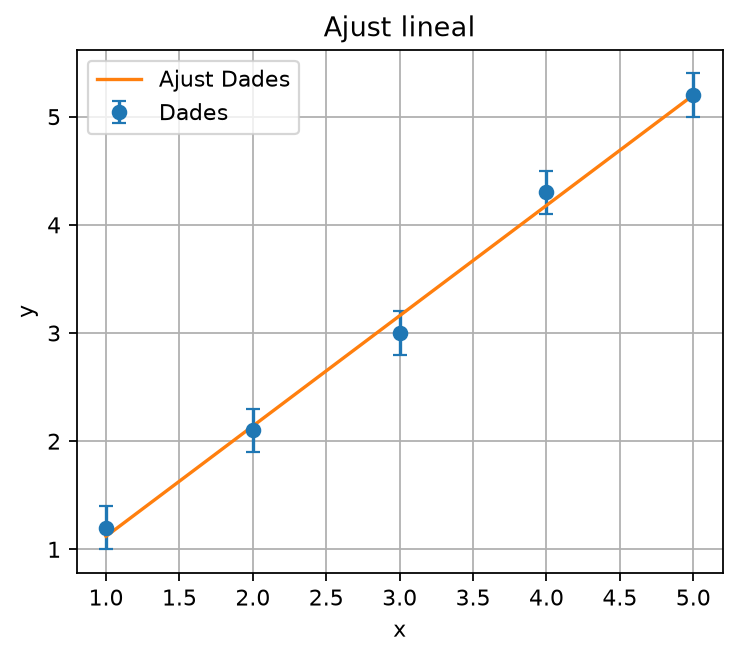
\includegraphics[width=0.7\textwidth]{fig1_lineal.png}
\caption{Gràfica de dades amb error i ajust lineal. La sortida simbòlica dels paràmetres es mostra separadament en executar el codi.}
\end{figure}

\subsection*{3. Ajust amb exclusió de punts i rang limitat}

\begin{lstlisting}
x, y, dy = llegeix_dades('Dades_Exemple/dades1.1.txt', skip=1)
mostra_dades(x, y, incert_y=dy, funcio_model=model_lineal, 
             titol='Ajust lineal eliminant algun punt i seleccionant el rang',
             xlabel='$Temps$ (s)', ylabel='$Distancia$ (m)',
             x_max=7, exclude=[9])
\end{lstlisting}

\begin{figure}[H]
\centering
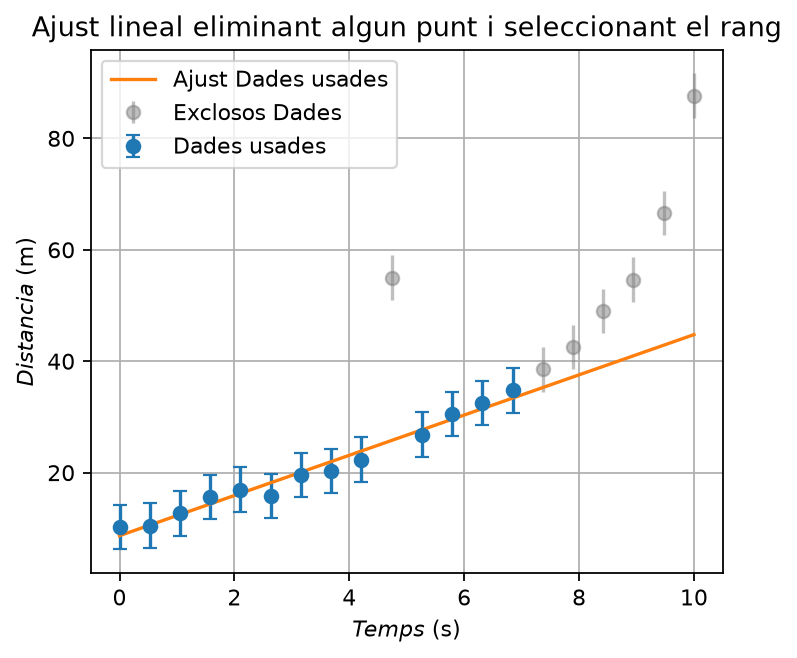
\includegraphics[width=0.7\textwidth]{fig2_exclosos.png}
\caption{Ajust lineal fins a $x=7$, amb exclusió del desè punt original. Els punts exclosos es mostren en gris.}
\end{figure}

\subsection*{4. Ajust exponencial}

\begin{lstlisting}
x = np . linspace (0 , 2 , 6)
y = np . array ([1.05 , 1.55 , 2.75 , 4.1 , 7.2 , 10.9])
dy = 0.1*y
mostra_dades (x , y , funcio_model = model_exponencial,
    incert_y = dy, titol = 'Ajust exponencial',
    xlabel = r'$t$ ( s )' , ylabel = r'$N$', log_y=True)
\end{lstlisting}

\begin{figure}[H]
\centering
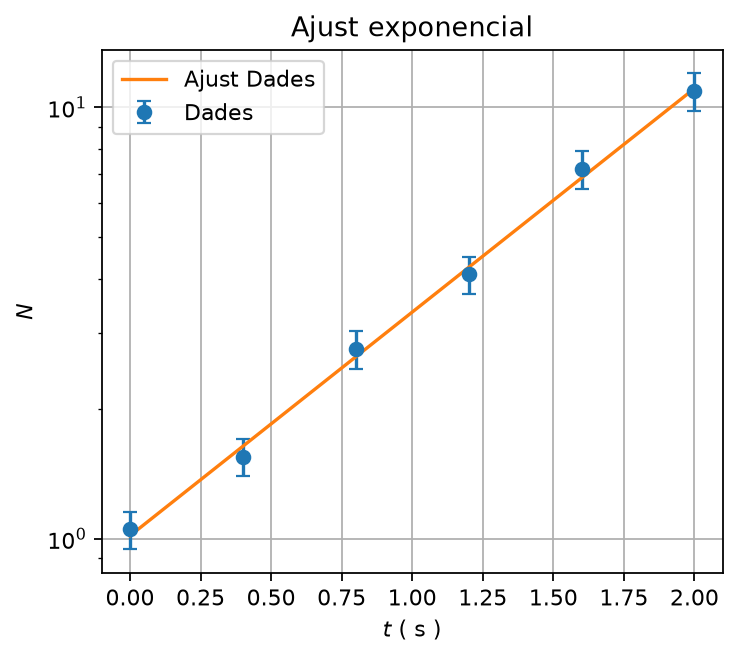
\includegraphics[width=0.7\textwidth]{fig3_exponencial.png}
\caption{Ajust a una funció exponencial \( y = a_0 e^{a_1 x} \) amb incerteses emprant escala logarítmica en l'eix vertical.}
\end{figure}

\subsection*{5. Ajust sinusoidal: importància dels valors inicials}

El model \(y=a_0\sin(a_1x+a_2)\) és no lineal en la freqüència angular
\(a_1\) i la fase \(a_2\). L'algorisme cerca un mínim local: una estimació
inicial inadequada pot conduir a una corba que no descriu les dades,
encara que el càlcul acabi sense errors. Això és diferent de no convergir.

Comparem els dos ajustos sobre les mateixes dades simulades. Sense
\texttt{valors\_inicials}, en aquest exemple els tres paràmetres parteixen
 del valor 1. En el segon intent proporcionem una estimació aproximada.

\begin{lstlisting}
x = np.linspace(0, 2*np.pi, 50)
np.random.seed(1)
y = 3*np.sin(2.5*x + 0.5) + np.random.normal(0, 0.3, len(x))

fig, axes = plt.subplots(1, 2, figsize=(10, 4),
                         constrained_layout=True)
ax0, r0 = mostra_dades(x, y, funcio_model=model_sinus,
                       ax=axes[0])
ax1, r1 = mostra_dades(x, y, funcio_model=model_sinus,
                       valors_inicials=[2, 3, 0], ax=axes[1])
axes[0].set_title('Valors inicials per defecte')
axes[1].set_title('Estimacions inicials [2, 3, 0]')
for ax in axes:
    ax.legend()
    ax.grid(True)
print('RMSE:', r0['rmse'], r1['rmse'])
\end{lstlisting}

\begin{figure}[H]
\centering
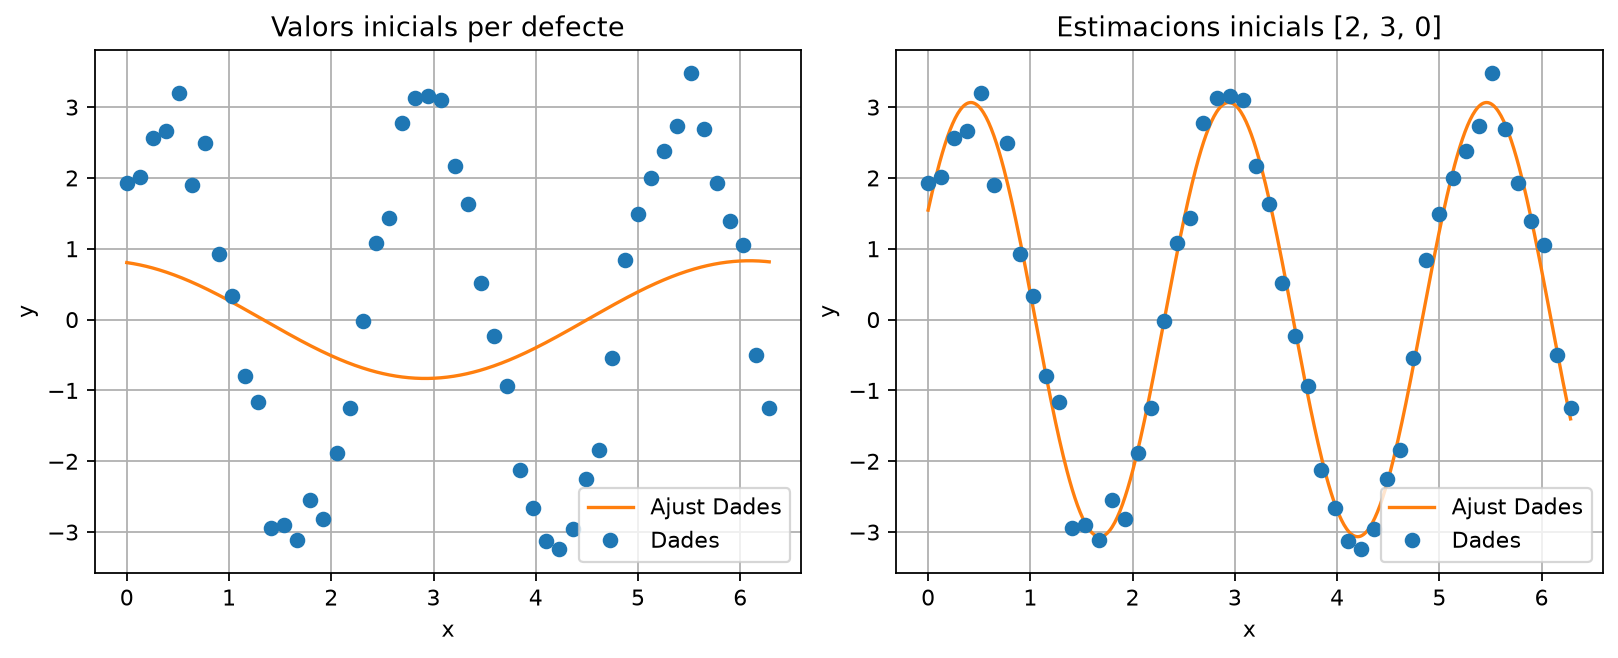
\includegraphics[width=\textwidth]{fig4_sin.png}
\caption{Les mateixes dades amb dues inicialitzacions. Amb els valors per
 defecte, l'ajust queda en una solució inadequada; amb una estimació
 inicial propera, recupera les oscil·lacions.}
\end{figure}

Per estimar els paràmetres a partir del gràfic, podem prendre l'amplitud
com la meitat de la diferència entre màxim i mínim i estimar el període
\(T\) entre dos màxims consecutius. La freqüència angular inicial serà
\(a_1\simeq2\pi/T\); la fase es pot estimar a partir de la posició d'un
màxim o d'un pas per zero. No cal conèixer els valors exactes.

Convé provar diverses estimacions plausibles, inspeccionar els residus
i comparar l'RMSE sobre les mateixes dades. Un RMSE petit, per si sol,
no demostra que el model sigui físicament correcte ni garanteix haver
trobat el mínim global. En aquest exemple no s'han proporcionat incerteses,
per la qual cosa comparem l'RMSE i no interpretem el camp
\texttt{chi2\_reduced} com un $\chi^2$ estadístic.

\subsection*{6. Exemple amb \texttt{mostra\_varies\_series}}
Permet representar diverses sèries de dades en una mateixa figura, amb ajustos independents. A cada sèrie li podem posar les mateixes opcions que a la funció \texttt{mostra\_dades}. 

Els paràmetres \texttt{titol}, \texttt{xlabel}, \texttt{ylabel} i \texttt{mida\_figura}, en cas que es vulguin especificar, s'han de passar al final perquè són comuns a tota la figura.

\begin{lstlisting}
import numpy as np
from funcions_labs import mostra_varies_series, model_lineal

np.random.seed(1)
x1 = np.linspace(0, 10, 20)
y1 = 2.0 * x1 + 1.0 + np.random.normal(0, 1, len(x1))
dy1 = np.full_like(x1, 0.5)

x2 = np.linspace(0, 10, 15)
y2 = -1.0 * x2 + 12.0 + np.random.normal(0, 1, len(x2))

series = [
    {"x": x1, "y": y1, "incert_y": dy1,
     "funcio_model": model_lineal,
     "label_dades": "Serie 1", "forma": "o", "color": "blue"},
     
    {"x": x2, "y": y2,
     "funcio_model": model_lineal,
     "label_dades": "Serie 2", "forma": "s", "color": "red"}
]

mostra_varies_series(series, xlabel="Variable X", ylabel="Variable Y",
                     titol="Exemple amb dues series")
\end{lstlisting}

La figura obtinguda mostra les dues sèries de dades amb els seus ajustos lineals respectius:

\begin{center}
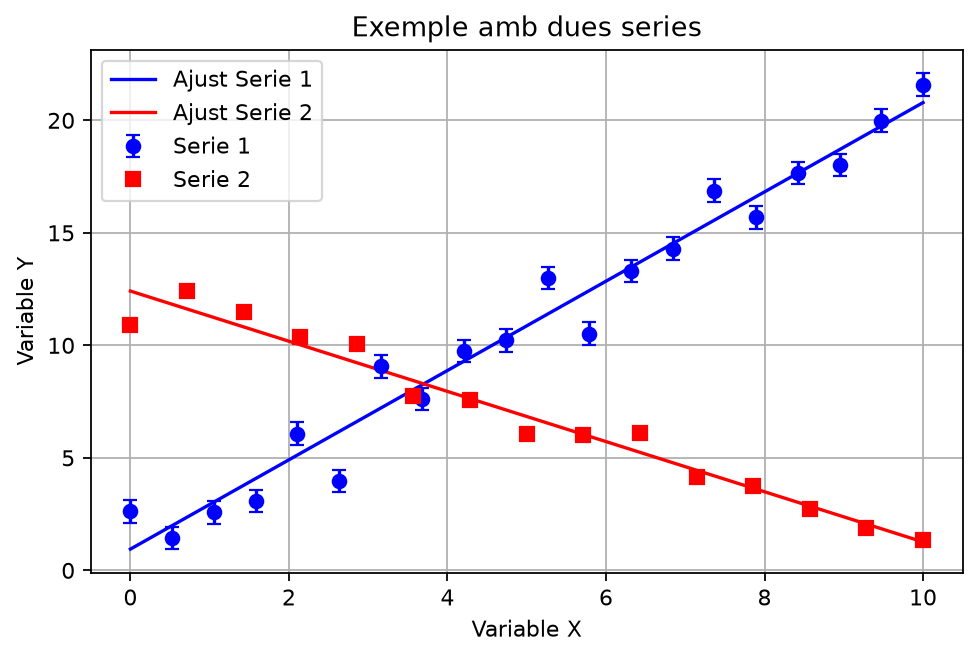
\includegraphics[width=0.8\textwidth]{exemple_varies_series.png}
\end{center}



\end{document}
